\documentclass[a4paper, 12pt, one column, aas_macros]{article}

\usepackage[italian]{babel}
\usepackage[utf8x]{inputenc}
\usepackage[T1]{fontenc}

\usepackage[top=1.3cm, bottom=2.0cm, outer=2.5cm, inner=2.5cm, heightrounded,
marginparwidth=1.5cm, marginparsep=0.4cm, margin=1.5cm]{geometry}

\usepackage{graphicx}
\usepackage[colorlinks=False]{hyperref} 
\usepackage{amsmath}  
\usepackage{amsfonts} 
\usepackage{amssymb}
\usepackage{fancyvrb}  

\usepackage[authoryear]{natbib}
\bibliographystyle{abbrvnat}
\setcitestyle{authoryear,open={(},close={)}}

\usepackage{pdfpages}
\usepackage{graphicx}
\usepackage{subfigure}
\usepackage{array}
\usepackage{siunitx}
\usepackage{booktabs}

\title{PasswordCollector, un'applicazione in Java per la gestione locale delle proprie password}
\author{Lorenzo LEONI}
\date{%
	Università degli studi di Bergamo, Dipartimento di Ingegneria Gestionale, dell'Informazione e della Produzione\\[2ex]%
	\today
}

\begin{document}
	\maketitle
	
	\section{Introduzione}
	Spesse volte ci si trova nella situazione di dover scrivere le proprie password su un foglio cartaceo perché malfidenti nei confronti dei servizi di archiviazione online, i quali si appoggiano a server che frequentemente sono vittima di hacker desiderosi di violare la nostra privacy. PasswordCollector cerca di ovviare a questa problematica fornendo un servizio di \textbf{gestione}, di \textbf{memorizzazione} e di \textbf{crittografia} delle password completamente locale. Nello specifico:
	\begin{itemize}
		\item l'archiviazione dei dati personali avviene tramite documenti JSON, un formato di interscambio che facilita la portabilità non solo dei contenuti informativi, ma anche dell'applicazione, di conseguenza;
		\item la cifratura dei dati sensibili avviene mediante una versione modificata del cifrario di Cesare. Esso si basa su uno spostamento causale in tabella ASCII delle lettere costituenti la password da mascherare;
		\item l'interazione e la gestione di PasswordCollector avviene tramite un'interfaccia a riga di comando.
	\end{itemize}
	Da sottolineare, infine, la possibilità di registrare più account in modo tale che la stessa istanza dell'applicazione possa essere utilizzata da più utenti senza che l'uno possa accedere ai contenuti dell'altro.
	
	\section{Funzionalità}
	PasswordCollector prevede \num{2} tipologie di account, le quali si distinguono per le funzionalità accessibili e per i privilegi.
	\begin{itemize}
		\item \textbf{user}: oltre al poter eliminare il proprio account e modificarne le informazioni quali, per esempio, indirizzo di posta elettronica e numero di telefono, un utente \textit{standard} ha soltanto la possibilità di inserire e visualizzare le proprie password, mentre un utente \textit{premium} può anche modificarle ed eliminarle. Questa differenziazione è stata inserita in modo tale da permettere un successivo inserimento di un sistema di monetizzazione;
		\item \textbf{administrator}: l'amministratore è unico, può disinstallare l'applicazione e visualizzare la lista degli utenti registrati. Inoltre, ha la possibilità di generare e gestire le \textit{premium key}, ossia un codice da associare a un indirizzo di posta elettronica. In fase di registrazione il nuovo utente può inserire una \textit{premium key}: se il codice esiste ed è associato all'indirizzo email fornito, allora le funzionalità premium vengono abilitate, altrimenti viene creato un account \textit{standard}.
	\end{itemize}
	Tutti i dati sensibili vengono crittografati e memorizzati in file JSON appartenenti a una cartella nascosta, ossia una directory non accessibile a occhi indiscreti. Solo gli utenti e l'amministratore sono a conoscenza della locazione del file system in cui la cartella \textit{Pw\_C0ll3ct0r} si trova.
	
	\section{Descrizione dei package e delle classi}
	Il codice sorgente dell'applicazione è distribuito in \num{3} package con l'obiettivo di raggruppare funzionalità simili e dipendenti tra di loro e di realizzare l'information hiding:
	\begin{itemize}
		\item package \textbf{encryptors} (figura \ref{UML_ecryptors});
		\item package \textbf{accounts} (figura \ref{UML_accounts});
		\item package \textbf{application} (figure \ref{UML_application_1} e \ref{UML_application_2}).
	\end{itemize}
	
	\subsection{Package encryptors}
	Contiene le classi \verb|CaesarEncryptor| e \verb|ModCaesarEncryptor|, le quali implementano rispettivamente il cifrario di Cesare e la sua versione modificata. La seconda estende la prima, che a sua volta implementa l'interfaccia \verb|EncryptorMethods|. Nel diagramma delle classi non è specificato, ma sia il metodo \verb|encrypts| sia \verb|decrypts| ricevono (implicitamente) in ingresso un array di stringhe tramite l'operatore \verb|varargs|.
	\begin{figure}[h!]
		\centering
		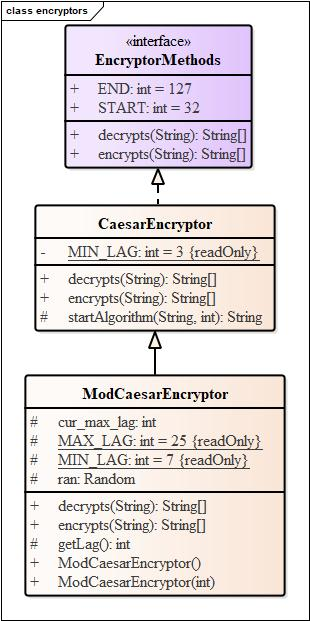
\includegraphics[height=300px]{UML/encryptors.jpg}
		\caption{diagramma UML delle classi relativo al package \textit{encryptors}.}
		\label{UML_ecryptors}
	\end{figure}
	
	\subsection{Package accounts}
	La classe astratta \verb|Account| serve per definire i metodi e i campi comuni a tutte le classi che da essa derivano, ossia \verb|AdminAccount| e \verb|UserAccount|, classe base di \verb|PremiumUserAccount|. \verb|AdminAccount| possiede una \verb|KeysCollection|, ovvero un oggetto che permette di accedere e gestire una lista di \verb|PremiumKey|. \verb|PremiumUserAccount|, invece, implementa l'interfaccia \verb|PwMethods| poiché l'utente \textit{premium} è l'unico avente il privilegio di modificare ed eliminare le proprie password; esse sono conservate durante l'esecuzione in una lista di \verb|Password|, il cui riferimento è memorizzato in \verb|PwList|, un campo ereditato dalla classe padre \verb|UserAccount|. Da notare, infine, l'enumerazione \verb|AccountTypes|: essa viene utile ogniqualvolta si vuole verificare la tipologia di un oggetto che rappresenta un utente senza ricorrere all'operatore \verb|instanceof|.
	\begin{figure}[h!]
		\centering
		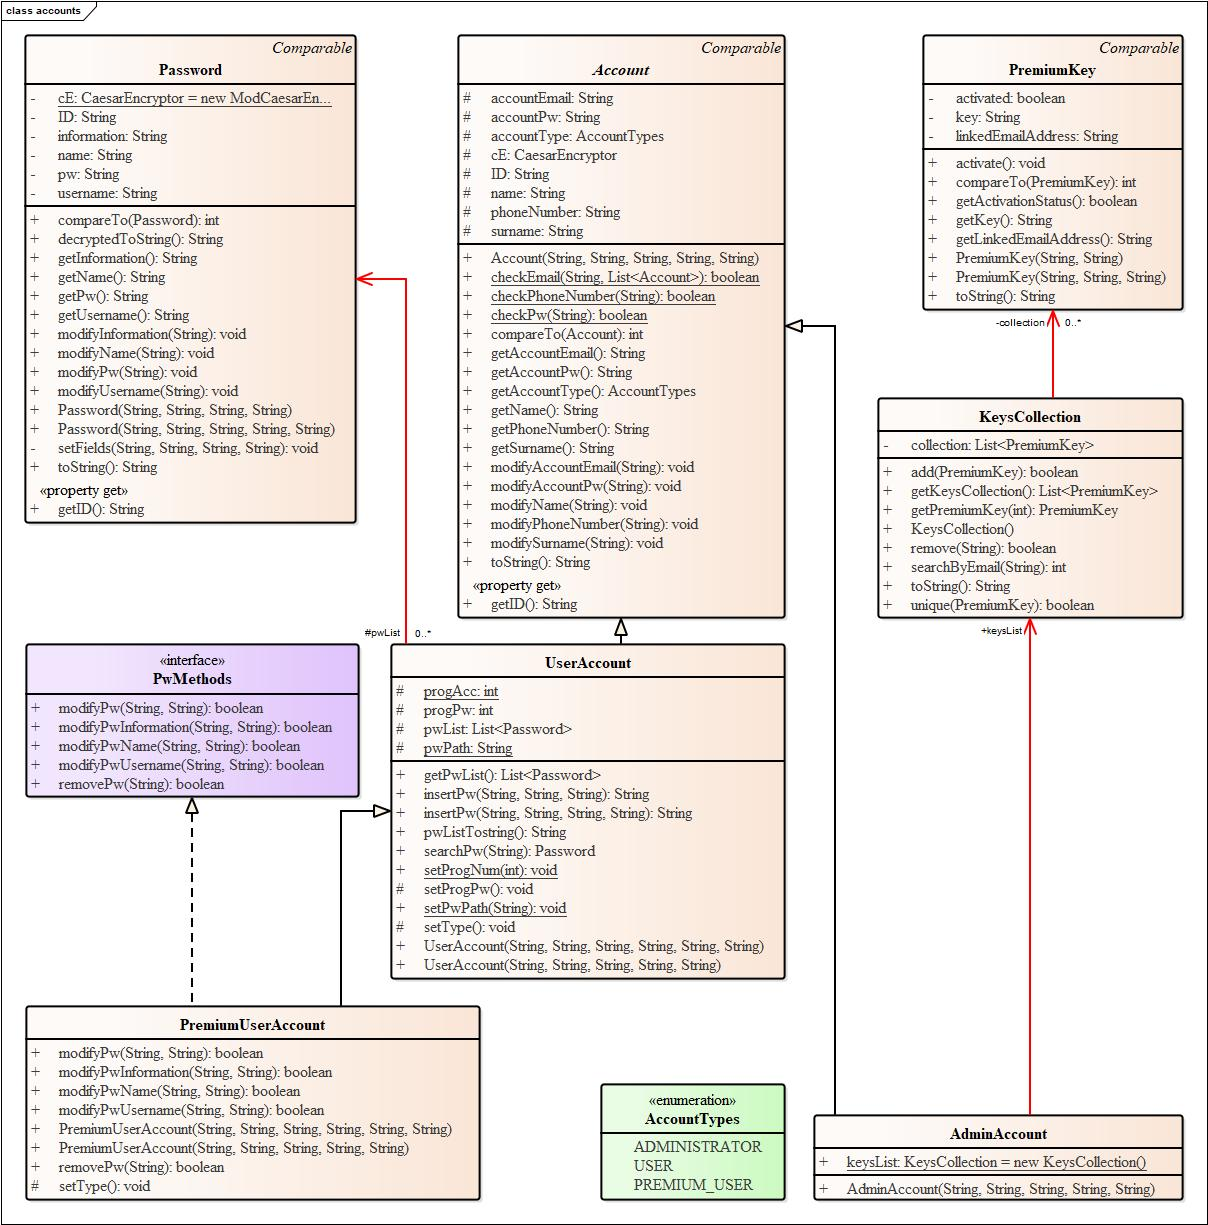
\includegraphics[height=500px]{UML/accounts.jpg}
		\caption{diagramma UML delle classi relativo al package \textit{accounts}.}
		\label{UML_accounts}
	\end{figure}
	
	\subsection{Package application}
	La classe \verb|Application| è il cuore di PasswordCollector, ossia l'hub dal quale è possibile accedere a tutte le funzionalità. Essa implementa le istanze di \verb|AccountHandler| e \verb|PasswordHandler|, le classi aventi il compito di invocare i metodi rispettivamente di gestione dell'account (compresi il login/logout e la creazione di un nuovo profilo) e delle sue password. In \verb|Application| è contenuto anche un oggetto appartenente alla classe \verb|AppData|, i cui campi contengono i path delle cartelle contenute in \textit{Pw\_C0ll3ct0r} e alcune informazioni riguardanti l'installazione. Invece, le classi \verb|Installer| e \verb|Initializer| contengono i metodi statici che vengono eseguiti rispettivamente per installare l'applicazione e per inizializzare le strutture dati \verb|accountList| e \verb|data| di \verb|Application| a partire dai documenti JSON nell'istante in cui PasswordCollector viene avviata. Non è possibile eseguire più applicazioni, quindi l'unica istanza di \verb|Application| avviabile è contenuta nella classe \verb|Singleton|. Infine, \verb|Util| implementa una serie di funzioni statiche per la lettura e per la scrittura da file.
	\begin{figure}[h!]
		\centering
		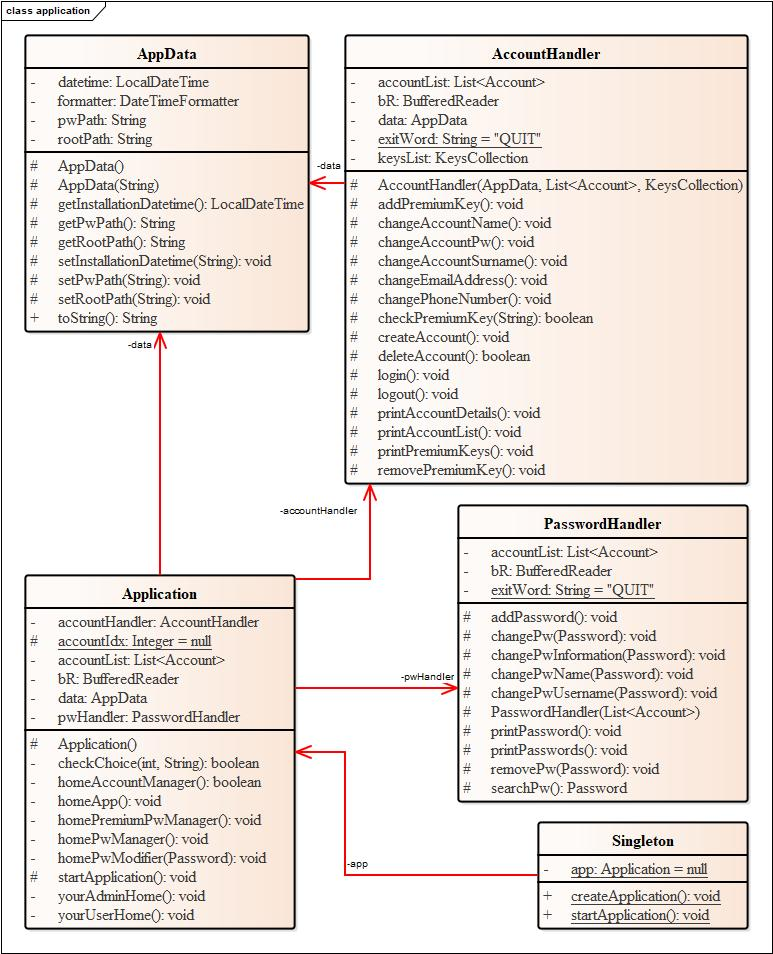
\includegraphics[height=450px]{UML/application1.jpg}
		\caption{diagramma UML delle classi relativo al package \textit{application}, parte \num{1}.}
		\label{UML_application_1}
	\end{figure}
	\begin{figure}[h!]
		\centering
		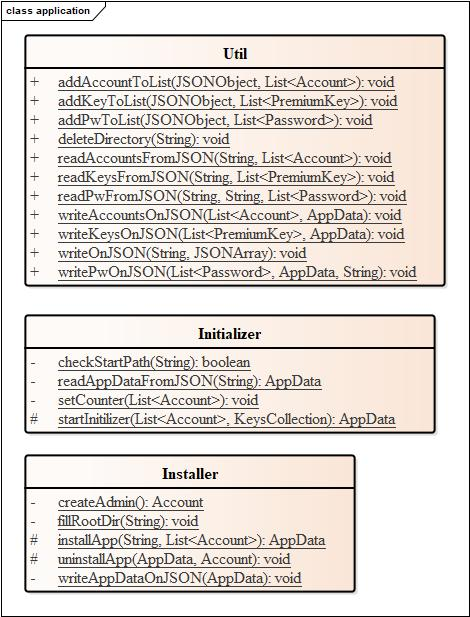
\includegraphics[height=300px]{UML/application2.jpg}
		\caption{diagramma UML delle classi relativo al package \textit{application}, parte \num{2}.}
		\label{UML_application_2}
	\end{figure}
	
	\section{Documenti JSON}
	Di seguito sono riportate le tracce dei documenti JSON all'interno dei quali vengono memorizzati in maniera persistente i dati di PasswordCollector:
	\begin{itemize}
		\item \textbf{app\_data.json}: contiene i percorsi e la data di installazione dell'applicazione. Da sottolineare che JSON affianca al backslash anche lo slash normale in modo tale che il path possa essere interpretato da tutti i parser;
		\begin{Verbatim}[tabsize=1]
		[
			{
				"installationDetails":{
					"root_path":"C:\\Users\\loren\\Desktop\/Pw_C0ll3ct0r",
					"passwords_path":"C:\\Users\\loren\\Desktop\/Pw_C0ll3ct0r\/Collections",
					"installation_datetime":"2023\/04\/30 16:01:44"}
			}
		]
		\end{Verbatim}
	
		\item \textbf{premium\_keys.json}: contiene l'elenco delle coppie chiave-indirizzo delle \textit{premium key} generate dall'amministratore. Se il campo \verb|"activation_status"| è \verb|"true"|, allora l'utente il cui indirizzo di posta elettronica è \verb|"linked_email_address"| ha creato il proprio account utilizzando la chiave a lui riservata;
		\begin{Verbatim}[tabsize=1]
		[
			{
				"premiumKey":{
					"activation_status":"true",
					"linked_email_address":"~!$w ,!@~w! {CKKJRy\u007Fs{~@u!\u007F\\",
					"key_value":"PcP[P]cP<@H?FM"}
			},
			{
				"premiumKey":{
					"activation_status":"false",
					"linked_email_address":"k{~wx7kj{krn{rI}r|ljur7r}\/",
					"key_value":"LrjxxjrLh;9;<\/"}
			}
		]
		\end{Verbatim}
	
		\item \textbf{accounts\_data.json}: contiene l'elenco di tutti gli account che sono stati creati. Da notare che le informazioni sensibili sono state criptate utilizzando la versione modificata del cifrario di Cesare;
		\begin{Verbatim}[tabsize=1]
		[
			{
				"account":{
					"account_email":"}?}v \u007FzCQ$%&uv\u007F%z?&\u007Fzsx?z%W",
					"account_type":"ADMINISTRATOR",
					"account_ID":"AD_0",
					"surname":"Leoni",
					"account_pw":"Puz{o{9@<<>",
					"name":"Lorenzo",
					"phone_number":";<?==88;88*"}
				},
				{
					"account":{
						"account_email":"} #v\u007F+ ?}v \u007FzBJJIQx~rz}?t ~W",
						"account_type":"PREMIUM_USER",
						"account_ID":"US_1",
						"surname":"Leoni",
						"account_pw":"X}\"#w#AHDHf",
						"name":"Lorenzo",
						"phone_number":"BCFDD??B??M"}
					},
					{
						"account":{
							"account_email":"&#v-B+|}(yT{!u} Bw#!f",
							"account_type":"USER",
							"account_ID":"US_2",
							"surname":"Bianchi",
							"account_pw":"ZyzzHHw99z",
							"name":"Roberto",
							"phone_number":"LNRRJKPNMO\u007F"}
					}
				]
		\end{Verbatim}
	
		\item \textbf{pw\_US\_1.json}: contiene l'elenco delle password e le informazioni a esse associate dell'account avente l'identificativo US\_1. Se il campo \verb|"information"| è \verb|"empty field"|, allora significa che l'utente non ha voluto specificare alcun dettaglio aggiuntivo per la password corrispondente. 
		\begin{Verbatim}[tabsize=1]
		[
			{
				"password":{"pw":"WD!$&Dh)(((D5FDFDf",
				"name":"Amazon.it",
				"information":"empty field",
				"ID":"PW_0",
				"username":"!v\"{z'\/$#k"}
			},
			{
				"password":{"pw":"k$!v'zzHBGEGH6k",
				"name":"Navigraph.com",
				"information":"Navigraph.com is a 
						web site where you can create 
						a Flight Plan (FP) for FS2020",
				"ID":"PW_1",
				"username":"%~!$)az$NMk"}
			}
		]
		\end{Verbatim}
	\end{itemize}

	\section{Versione modificata del cifrario di Cesare}
	L'algoritmo di Cesare consiste nello spostare in avanti di \num{3} posizioni ogni lettera di una parola, riferendosi alla tabella ASCII. Per esempio, "\textbf{Lorenzo-1998}" diventa "\textbf{Oruhq\}r04<<;}". Nella sua versione modificata, invece, lo spostamento ($lag$) è scelto casualmente tra \num{7} e \num{25} (\num{15} in PasswordCollector). Tuttavia, per decifrare la parola è necessario conoscere il $lag$, pertanto in coda a essa viene aggiunto un carattere dal quale è possibile risalire allo spostamento casuale generato dall'algoritmo. Le formule di cifratura e di decifrazione del $lag$ sono rispettivamente:
	\begin{verbatim}
		char charLag = (char) (lag*5 + 2)
		lag = ((int) charLag - 2)/5
	\end{verbatim}
	dove \verb|charLag| rappresenta il simbolo in tabella ASCII la cui posizione risulta dall'applicazione della formula al \verb|lag|. Se lo spostamento vale \num{7}, allora $7\cdot5 + 2 = 37$, il quale corrisponde al simbolo "\%" in tabella ASCII. Se, invece, il $lag$ è uguale a \num{25}, allora $25\cdot5 + 2 = 127$; esso coincide con l'ultimo simbolo utilizzabile in quanto, per questioni rappresentative e di codifica, è stato deciso di utilizzare soltanto i simboli in tabella ASCII che vanno dalla posizione \num{32} alla \num{127}. Di seguito è riportato un esempio di decifrazione di una password criptata:
	\begin{center}
		"\textbf{]vshyll:4979:(\%}"\\
		"\textbf{\%}" corrisponde a \num{37} in tabella ASCII\\
		$lag$ = $(37-2)/5$ = 7\\
		\num{-7} per ogni carattere: "\textbf{Volaree3-2023!}"
	\end{center}
	
	\section{Repository GitHub}
	Il codice sorgente di PasswordCollector è disponibile per il download al seguente repository:
	\begin{center}
		\url{https://github.com/lamferzon/PasswordCollector}
	\end{center}
	\begin{figure}[h!]
		\centering
		\subfigure[]{\label{Screen1}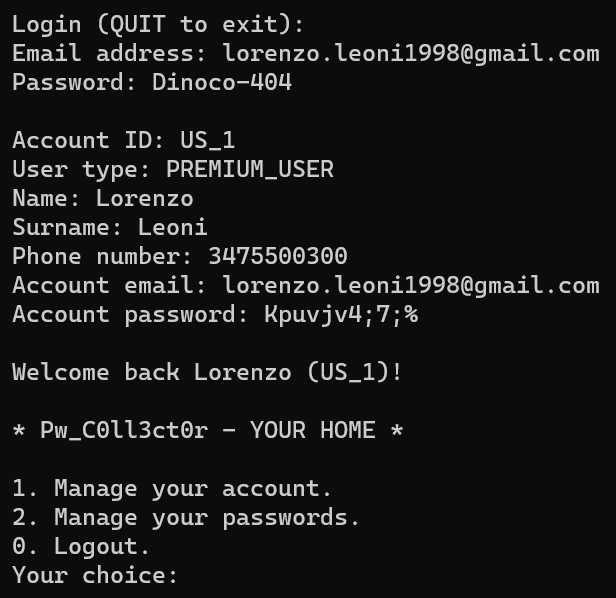
\includegraphics[height=200px]{Immagini/Screenshot1.jpg}}
		\subfigure[]{\label{Screen2}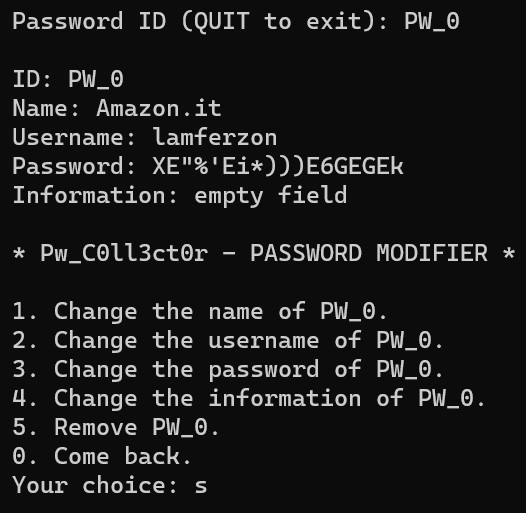
\includegraphics[height=200px]{Immagini/Screenshot2.jpg}}
		\caption[]{un paio di screenshot dell'applicazione in esecuzione.}
		\label{App_screens}
	\end{figure}
	
\end{document}